\documentclass{article}
\usepackage[utf8]{inputenc}

\usepackage[a4paper]{geometry}

\usepackage{amsmath}
\usepackage{amsthm} % theorems, definitions etc.

\usepackage{hyperref} % hyperlinks and pdf contents

\usepackage{graphicx}
\DeclareGraphicsExtensions{.png,.pdf}
\graphicspath{{images/}}

\title{Bachelor}
\author{Andreas Matre}
\date{February 2020}

\begin{document}

\newtheorem{definition}{Definition}[section]
\newtheorem{theorem}{Theorem}
\newtheorem{example}{Example}[section]


\maketitle

\begin{abstract}
 test 
\end{abstract}

\tableofcontents

\section{Introduction}

Linear regression is a useful tool to describe relationships between variables.
When we want to investigate possible accosiations, linear regression
is one of the most common tools we could use. It can be used to show show correlation between
variables, and in some cases where experiments are designed very carefully, it can even suggest causation.
It can for example be used in the social sciences to try to show a relationship
between income and age of death.
When fitting a model, data is needed. It is very important to take into account the methods used in
the information gathering when fitting models.

One needs some kind of ``randomness'' to do statistics. There are different
approaches to get this.
One of them is that one assumes that the population sampled from is part of a ``superpopulation'', i.e. an
infinite population, that has some distribution. This could for example be a
normal distribution with some mean and variance.  This distribution is where the
``randomness'' comes from. In this case the way the data
is collected is not that important. This is called a model based approach.

An other approach is to not assume that the population you sample is part of a
superpopulation, and therefore does not have a distribution either.
One instead samples from a finite population and the ``randomness'' comes from
considering the probability of each individual in the population being included
in the sample. This is a design based approach and is what survey statistics is about. Here it's more important how
you collect the data.
The goal of survey statistics is to be able to do statistical analysis without
making assumptions with regards to the distribution of the data. The advantage
of not making these assumptions is that we don't risk them being wrong, which
would weaken the confidence in the results. On the other hand,
making these assumptions allows us to decrease the variance as the assumptions
gives the data some structure. By making as few assumptions as possible we
therefore get larger variances and more uncertainty.

This thesis shows how to fit
a linear regression model when data is collected through a complex survey design, i.e,
a survey including unequal sampling probabilities, stratification, which is when we
create a partition of the population and then sample from each subset, and
clustering, where we again create a partition of the population but here, which
of these subsets we sample from is also random.
To do analysis in these cases weights are used. Each observation gets a weight
value which can be interpreted as the number of individuals in the population
that observation represents. So an observation with a small chance of being
included in the sample would have a larger weight than one with a high chance of
being included.
In normal regression each individual in the population has the same chance of
being included so each observation therefore has the same weight.

One of the big problems of doing analysis on data collected through complex
survey designs is the fact that calculating variances can be extremely
difficult. One therefore often end up having to estimate the variance through
various techniques instead of calculating it exactly.
The fact that we have a finite population also influences the variance, since we
get something called the finite population coefficient. This is a factor \(1 -
\frac{n}{N}\), where \(n\) is the size of the sample and \(N\) is the size of
the population. This factor takes into account the fact that as we get a larger
and larger sample we can learn everything about the population, and therefore
the variance goes to zero.

We start
with an example illustrating what can go wrong if the methods used in the
information gathering is not taken into account.


\begin{example}

We will use a dataset from a study of the relationship between the length of a persons left middle finger and their height. 
The researcher oversampled people having short fingers and undersampled people
having long fingers.
The dataset contains 200 samples, each containing the length of the persons left middle finger (cm), their height (cm) and the probability that they would be chosen for the sample.

To illustrate the difference, the left panel in Figure \ref{fig:anthSamples} shows a random sample where every
person had an equal chance of being included. While the right panel in Figure \ref{fig:anthSamples} shows a sample
where short people had a higher chance of being included than tall people. The
observations in the right panel is much more concentrated in the bottom.

\begin{figure}
  \label{fig:anthSamples}
  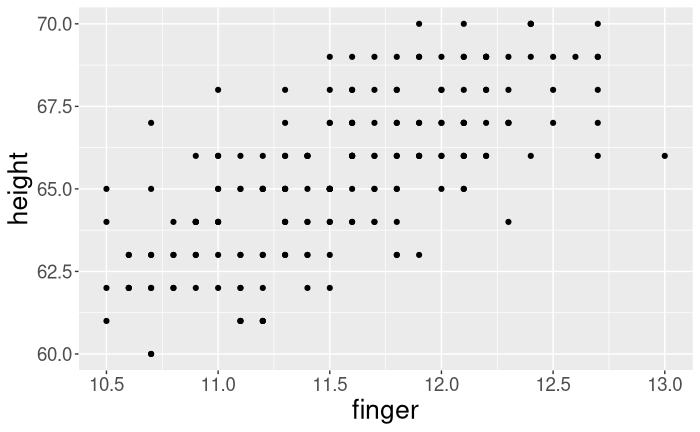
\includegraphics[scale = 0.4]{example1_SRS.png}
  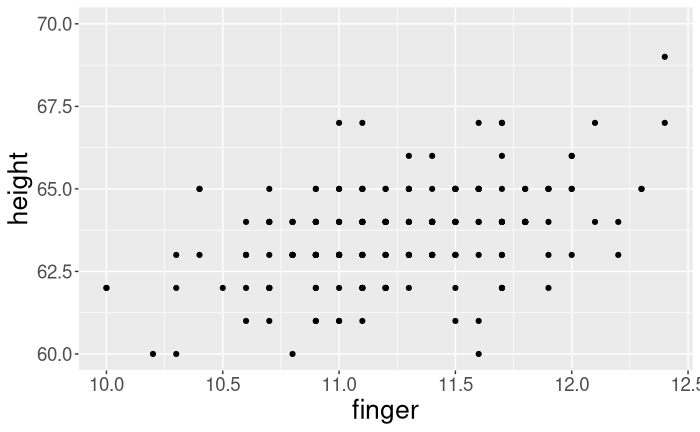
\includegraphics[scale = 0.4]{example1_UNEQ.png}
  \caption{Two samples of finger length versus height. Left: Every person has the same
    probability of being included in the sample. Right: The probability of being
  included in the sample depends on height.}
\end{figure}


This means that fitting a linear regression model to the unequal probabilities
sample will result in the slope tending to be smaller than what it should be, since there are few observations in the top right of the plot.

This will be illustrated now by fitting both a naive linear model and a model that takes into account the sampling probabilities.

% Code and plot of regression lines
%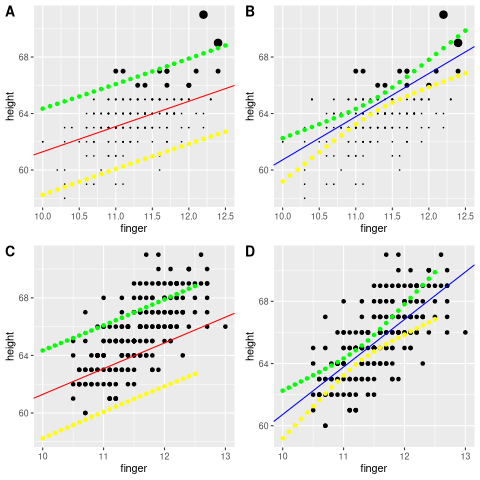
\includegraphics[scale = 0.5]{example1.png}

\begin{figure}
  \centering
  
  \includegraphics[scale = 0.5]{ex1Pred}
  \includegraphics[scale = 0.5]{ex1Pred2}
  \caption{Plots showing regression lines for equalprobability and
    unequalprobability samples and linear regression with and without taking the
    sampling probabilities into account. Top plots are the unequal probability
    sample where short people are oversampled. Bottom plots are the equal
    probability sample where every person has the same chance of being included
    in the sample. Solid lines are the prediction lines which the dashed lines
    represent the
    95\% prediction interval. Red lines are for normal regression which blue
       lines are for regression taking sampling probabilities into account.}
  \label{fig:ex1Pred}
\end{figure}

\textbf{I Figur \ref{fig:ex1Pred} synes jeg plottet med både blå og røde linjer i samme plott virker litt
  uoversiktlig, så burde kanskje gå for det med alle fire plottene?}

Figure \ref{fig:ex1Pred} shows the difference between taking into account the
sampling probabilities or not.
In the top plots, where the regression lines are plotted on top of the unequal
probability sample we can see that the line from normal linear regression, which
is the red line, fits very well with the sample. While the line from linear
regression taking into account the unequal sampling probabilities, the blue line, seems to be a
bit too steep.

When we look at the bottom plots however which show the regression lines on top
of a sample where every one has equal sampling probabilities however we see that
the line using normal linear regression, red line, is way too flat, while the
one taking into account the sampling probabilities fits much better.
By looking at the dashed lines which is a 95\% prediction interval we see that
the prediction interval from the normal linear regression does not seem to
include 95\% of the observations, while the one from the linear regression
taking into account the sampling probabilities does.
\end{example}

The examples illustrating the theory are focused on one dataset. This is a dataset on the performance of students in schools in
California. The dataset has data on all 6194 schools having more than 100
students in California, with data collected
including: API scores in 1999 and 2000, which level of school it is
(elementary, middle, high), name of school, location of school, percentage of
students tested at the school, API targets, economic factors for students at the
school, class sizes, information of education of parents and qualification of teachers.
API scores is a metric testing the academic performance of the students at the school.
We will use this data as the population we will sample from, and we will take
different kinds of samples to illustrate the concepts introduces in this thesis.

%The thesis will start by giving an introduction to survey statistics, where giving the necessary background theory needed to be able to talk about linear regression in this context.

\section{Model based simple linear regression} \label{sec:modLinReg}

We first give a short summary of classical simple linear regression. We have a response variable, \(y_i\), and a predictor,
\(x_i\) where \(i = 1, ..., N\), where \(N\) is the number of observations. The
relationship between the response and the covariates is assumed to be:

\begin{equation*}
Y_i = \beta_0 + \beta_1 x_i + \epsilon_i,\ i = 1, \dots, N
\end{equation*}
where \(\epsilon_i\) is a stochastic error term with some distribution. We
assume \(\beta_0\) and \(\beta_1\) are constants.

I.e, we assume there exists \(\beta_0\) and \(\beta_1\) that describes the
deterministic part of this relationship.
We do not know the values of \(\beta_0\) and \(\beta_1\), so we have to estimate them from observed data points. We call these data points \((x_1, y_1), (x_2, y_2)
... (x_N, y_N)\). To do
this we want to find \(\hat{\beta}_0\) and \(\hat{\beta}_1\) that minimize the
Residual Sum of Squared (RSS). The RSS is defined by:

\begin{align*}
  RSS &= \frac{1}{N} \sum_{i = 1}^N \left( y_i - \hat{y}_i \right)^2 
  = \frac{1}{N} \sum_{i = 1}^N \left( y_i - \hat{\beta}_0 - \hat{\beta}_1 x_i \right)^2
\end{align*}

The \(\hat{\beta}_0\) and \(\hat{\beta}_1\) that minimizes the RSS are:
%$$
%\hat{\beta}_1 = \frac{\sum_{i = 1}^N\left( x_i - \bar{x} \right) \left( y_i -
    %\bar{y} \right)} {\sum_{i = 1}^N \left( x_i - \bar{x} \right)}
%$$
%and
%$$
%\hat{\beta}_0 = \bar{y} - \hat{\beta}_1 \bar{x}
%$$

\begin{equation*}
 \hat{\beta}_1 = \frac{\sum_{i = 1}^N\left( x_i - \bar{x} \right) y_i}{\sum_{i = 1}^N\left( x_i - \bar{x} \right)} 
\end{equation*}

\begin{equation*}
 \hat{\beta}_0 = \bar{y} - \hat{\beta_1}\bar{x} 
\end{equation*}

Under the following conditions:

\begin{enumerate}
\item \(\mathrm{E} \left( \epsilon_i \right) = 0\ \forall \ i = 1, 2, ..., n\)
\item \(\mathrm{Var} \left( \epsilon_i \right) = \sigma^2\ \forall \ i = 1, 2, ..., n\)
\item All the \(\epsilon\) are independent of any predictor or observation number.
\item All \(\epsilon_1\), \(\epsilon_2\), ..., \(\epsilon_n\) are independent of each other.
\end{enumerate}

we get some useful properties, among which are these unbiased estimates for the
variance of \(\hat{\beta}_0\) and \(\hat{\beta}_1\):

\begin{equation*}
  \widehat{\mathrm{Var}} \left( \hat{\beta}_0 \right) = s^2 \frac{\sum_{i = 1}^N x_i^2}{n
    \sum_{i = 1}^N \left( x_i - \bar{x} \right)^2}
\end{equation*}
  

\begin{equation*}
  \widehat{\mathrm{Var}} \left( \hat{\beta}_1 \right) = \frac{s^2}{
    \sum_{i = 1}^N \left( x_i - \bar{x} \right)^2}.
\end{equation*}

Where \(s^2 = \frac{1}{N - 2} \sum_{i = 1}^N\left( y_i - \hat{\beta}_0 -
  \hat{\beta}_1 x_i \right)^2\) is an
unbiased estimator for the unknown \(\sigma^2\).

This is all based on the fact that the response has a distribution, which again
is based on the assumption that we have an infinite population to sample from.
What happens then, if we have a finite population? And what if the elements in
the sample are not independent of each other?

This is what survey statistics tells us.

\section{Introduction survey statistics}

\textbf{Slik som denne seksjonen er nå repeterer jeg litt det jeg skrev i
  introduksjonen om forskjellene mellom survey statistics og ``normal''
  statistikk. Burde jeg fjerne det jeg repeterer her eller er det greit å gjøre
  det?
Har ikke gått så nøye gjennom denne seksjonen ettersom jeg er usikker på hvor
mye som skal være med.}
There are two big differenses between ``normal'' statistics and Survey statistics.

The first difference is that in Survey statistics you approach the ''randomness'' from a different angle.
Usually in statistics you let individual values be stochastic variables
with some distribution and one observation is a sample from that stochastic
variable.

In Survey statistics on the other hand you say that the individual values are
fixed, i.e. my height is not random, every time you measure it you will get the
exact same result, if you discount measurement errors. Instead what is random is
who we sample. This leads us to a couple definitions:

\begin{definition} \label{def:sampUnitPopFrame}
  A \textbf{sampling unit} is one "element" we want to sample.
  The \textbf{sampling population}, or universe, \(U = \{1, 2, 3, ..., N\}\), is a
  finite set containing all the sampling units you are interested in. 
  The \textbf{sampling frame} is the list of all sampling units you are going to sample from. 
\end{definition}

In the case of our API example, our sampling units are schools, while
the sampling population is all the schools in California having more than 100 students.
The sampling frame would be all schools in California that the researchers know
about and that the researchers think have more the 100 students.
Ideally the sampling frame and the sampling population would be the same, but that is not always to case.

When taking different types of samples from the API dataset, the sampling population and the sampling frame are equal, since
we have a table of all the data and we will just choose rows from that table for
our samples. But there are cases where this is not the case. An example of this
could be if we were doing a political survey to try to predict who will win the
next election.
In that case our sampling population, who we are interested in information
about, would be everyone who are going to vote in the next election. It is
is impossible to get a list of them though, so we instead have to use 
some other part of the population we have information about. We might have a
list of all who voted last election, which might be a good approximation of
those who are going to vote this election, but then we would miss out on all the
new eligible voters and people who might have decided to vote this election but
didn't do it the last one.
Choosing the correct sampling frame to match your target sampling population is
difficult and getting it wrong will influence your results.

To represent the elements in \(U\) by natural numbers we let the elements
have a arbitrary ordering and denote them by their indices. We do this for
simplicity of notation as the order of the elements do not matter in the inference.


\begin{definition} \label{def:sample}
A \textbf{sample}, \(S \subseteq U\), is a subset of the sampling frame. This is the data we will analyse to try to get information about the sampling population.
A \textbf{probability sample} is a sample where the sampling units included are chosen randomly.
The \textbf{sampling probability} of a sampling unit is the probability that a specific sampling unit is included in the sample.
\end{definition}

We will denote the sampling units chosen in the sample by their indices in the
sampling population.

So we have a probability sample, where every sampling unit has some probability to be included in the sample, called the sampling probability.

\vspace{5mm}

The second big difference is that normally you assume that you sample from an
infinity population which has some distribution. In Survey statistics however we
have a finite distribution which means that it no longer makes sense thinking
about it having a distribution. This means that we no longer need the assumption
of which distribution the sampling units come from. This gives us more freedom,
and less potential problems if our assumptions are wrong.


The goal of Survey statistics is generally to estimate some statistic of the whole
population from a sample. These statistics include the total of some value,
f.eks. the total number of students in school, the mean of some value, f.eks.
the mean number of students per teacher in school, or to estimate regression
coefficients to either do inference or predict future values.

I will first start by talking about different kinds of samples along with some
inference on some statistics calculated from these samples and then finish with
talk about regression.


\section{Regression in the context of finite populations}
Now consider the case where the population is finite, i.e. we have \((x_1, y_1),
(x_2, y_2), \dots , (x_N, y_N)\), where the \(x_i\)'s are the covariates we use to
predict \(y_i\) and \(N\) is the size of the population.

Our goal in linear regression in this case is that we want to find the linear
line, \(y = B_0 + B_1x\), that best approximates this population. We define the best line as the one
that minimizes \(\mathrm{RSS} = \sum_{i = 1}^N (y_i - B_0 - B_1 x_i)^2\).
Minimizing the RSS means that we minimize the the squared distance of each point
in the population from the line.

In the case of finite populations, things change a bit. We still want to find the
coefficients that minimize the RSS, but since the population is finite our goal
is to estimate the line that minimizes the RSS for the whole population, i.e. find
\(B_0\) and \(B_1\) such that \(\sum_{i = 1}^N (y_i - B_0 - B_1 x_i)^2\) is as small as
possible.

If we know the whole population we can just compute \(B_0\) and \(B_1\) using the same formulas
as in Section \ref{sec:modLinReg}, which after rewriting them become:

\begin{equation*}
  B_0 = \frac{1}{N} \left( t_y - \frac{t_{xy} t_x - \frac{1}{N} t_y t_x^2}
    {t_{x^2} - \frac{1}{N} t_x^2}
   \right)
\end{equation*}

\begin{equation*}
  B_1 = \frac{t_{xy} - \frac{1}{N} t_y t_x}
    {t_{x^2} - \frac{1}{N} t_x^2}
\end{equation*}

where \(t_x = \sum_{i = 1}^N x_i\), \(t_y = \sum_{i = 1}^N y_i, t_{x^2} =
\sum_{i = 1}^N x_i^2\) and \(t_{xy} =
\sum_{i = 1}^N x_i y_i\).


The case where we know the whole population however is not that interesting, we are instead interested in the case where we have to sample from the
population to estimate such statistics.

If we then let \(\hat{t}_x, \hat{t}_y, \hat{t}_{x^2}, \hat{t}_{xy}, \hat{N}\) be estimators
for \(t_x, t_y, t_{x^2},
t_{xy}, N\) respectively, we get the estimators for \(B_0\) and \(B_1\):

\begin{equation*}
  \hat{B}_1 = \frac{\hat{t}_{xy} - \frac{1}{\widehat{N}} \hat{t}_y \hat{t}_x}
    {\hat{t}_{x^2} - \frac{1}{\widehat{N}} \hat{t}_x^2}
\end{equation*}

\begin{equation*}
  \hat{B}_0 = \frac{1}{\widehat{N}} \left( \hat{t}_y - \frac{\hat{t}_{xy} \hat{t}_x - \frac{1}{\widehat{N}} \hat{t}_y \hat{t}_x^2}
    {\hat{t}_{x^2} - \frac{1}{\widehat{N}} \hat{t}_x^2}
  \right)
  = \frac{\hat{t}_y}{\hat{N}} - \hat{B}_1\frac{\hat{t}_x}{\hat{N}}
\end{equation*}

To do this however we need to introduce some terminology:

Since \(\hat{B}_0\) and \(\hat{B}_1\) are non linear expressions of dependent
statistics, calculating exact variances can get very complicated. We therefore
often have to settle with having estimates of the variances instead.
There are several ways to do so, but a common one,
and the one we will use in here, is linearization. Linearization takes a
non-linear expression of stochastic variables we can do inference about and uses
the first two terms of the Taylor expansion to make it linear.
Say for example we have \(h(a, b, c, d, e) = \frac{ea - bc}{ed - b^2}\), such that
\(h(\hat{t_{xy}}, \hat{t_x}, \hat{t}_y, \hat{t}_{x^2}, \hat{N}) = \hat{B_1}\).
We then get:
\begin{align*}
  \mathrm{Var}(\hat{B_1})
  &= \mathrm{Var} \left( h(\hat{t_{xy}}, \hat{t_x},
  \hat{t}_y, \hat{t}_{x^2}, \hat{N})) \right) \\
  &\approx \frac{\widehat{\mathrm{Var}}\left( \sum_{i \in S} w_i q_i \right)}
    {\left( \sum_{i \in S} w_i x_i^2 - \frac{\left( \sum_{i \in S} w_i x_i \right)^2}{\sum_{i \in S} w_i} \right)^2}
\end{align*}

where \(q_i = (y_i - \hat{B}_0 - \hat{B}_1 x_i)(x_i - \hat{\bar{x}})\).

\subsection{Simple random sample}

One of the simpler probability samples is a Simple Random Sample (SRS). A
sample of size \(M \leq N\) is an SRS if every subset \(S \subseteq U\) has the same
probability of being chosen.
Say for example that \(U = \{1, 2, 3, 4\}\) and that we want a sample, \(S\) of
size \(3\). Then there are \(\binom{4}{3} = 4\)  possible samples:
\begin{equation*}
 S_1 = \{1, 2, 3\}, 
 S_2 = \{1, 2, 4\}, 
 S_3 = \{1, 3, 4\}, 
 S_4 = \{2, 3, 4\} .
 \end{equation*}

%\( S_1 = \{1, 2, 3\} \)
%\( S_2 = \{1, 2, 4\} \)
%\( S_3 = \{1, 3, 4\} \)
%\( S_4 = \{2, 3, 4\} \).

For this to be a SRS each of these subsets need to have the same probability of
being chosen, i.e. \(P(S_1) = P(S_2) = P(S_3) = P(S_4) = 0.25\). A consequence of
having a SRS is that all the sampling probabilities are equal, \(P(1 \in S) =
P(2 \in S) = P(3 \in S) = P(4 \in S) = 0.75\). But having equal sampling
probabilities is not sufficient for the sample to be an SRS.
Look for example at this case:
Assume we want a sample of size \(2\) from a population of size \(4\), and that
\(P(\{1, 3\}) = 0.5\) and \(P(\{2, 4\}) = 0.5\) while the probabilities of all the
other possible samples are \(0\). Then \(P(1 \in S) = P(2 \in S) = P(3 \in S) = P(4 \in S) = 0.5\)
but this is not a SRS since all possible subsets of size \(2\) do not have equal
probability of being chosen.


\subsection{Estimation}

One of the more common statistics we want to estimate is the total of some value
for the whole population. We might for example want to estimate the total number
of students enrolled in school, in our API example.

We would then denote the value of interest in one school, i.e. the number of
enrolled students by \(y_i\) and let
\(
  t_y = \sum_{i = 1}^{N} y_i
\)
be the value we want to estimate.
The natural estimate of this total, if we sample \(n\) elements, would be
\(
\hat{t}_y = \frac{N}{n}\sum_{i \in S} y_i
\)
where we take the average of the values in our sample and then scale it up to
the whole population.
It can be shown using indicator variables and sampling probabilities that
\(\hat{t}_y\) is an unbiased estimator for \(t_y\).
%A statistic related to the total is the mean of some value. We denote the true
%mean in the population
%\begin{equation*}
%\bar{y}_U = \frac{1}{N} \sum_{i = 1}^{N} y_i
%\end{equation*}
%and the sample mean
%\begin{equation*}
%\bar{y}_S = \frac{1}{n} \sum_{i \in S} y_i ,
%\end{equation*}
%which we use as our estimator.
%
%Then we can rewrite the estimate for \(t\) as:
%\begin{equation*}
%\hat{t}_y = \frac{N}{n} \sum_{i \in S} y_i = N\bar{y}_S
%\end{equation*}
%
%Using the fact that \(\hat{t}_y\) is unbiased it is trivial to show that
%\(\bar{y}_S\) is an unbiased estimator for \(\bar{y}_U\).
It can also be shown that the variance of the estimator is of the form:
\begin{equation*}
\mathrm{Var} \left( \hat{t}_y \right) = S^2\frac{N^2}{n} \left( 1 - \frac{n}{N}
\right)
\end{equation*}

where
\(
S^2 = \frac{1}{N - 1} \sum_{i = 1}^N (y_i - \bar{y})^2
\)
is the variance of the whole population.
We do not, however, know \(S^2\) as that would require us to know the \(y\) values
for the whole population \(U\). Instead we estimate \(S^2\) by the unbiased estimator:
\(
  s^2 = \frac{1}{n - 1} \sum_{i \in S} \left( y_i - \hat{\bar{y}} \right)^2
\)
which gives us the estimate of \(\mathrm{Var}(\bar{y}_U)\):
\begin{align*}
  \widehat{\mathrm{Var}(\hat{t}_y)}
  &=\frac{N^2}{\left( n - 1 \right)n} \left( 1 - \frac{n}{N} \right) \sum_{i \in S} \left( y_i - \hat{\bar{y}} \right)^2
\end{align*}
Since \(s^2\) is unbiased we have that \(s^2\frac{N^2}{n} \left( 1 - \frac{n}{N}
\right)\) is an unbiased estimator of the variance of \(\hat{t}_y\).

We see that all these estimators for totals and means are the same as in the
model based case. Therefore the estimates for the coefficients in the regression
model are also the same. The variance of the estimators for the coefficients are
different however.
The factor \(\left( 1 - \frac{n}{N} \right)\) in the variances is what differs in
the variance estimate compared to the model based one. It is called the
\textbf{finite population coefficient (fpc)} and comes from the fact that we are
sampling without replacement from a finite population.
When we sample a larger and larger portion on the population we will get more
and more information and therefore the variance will decrease towards zero.
This means that if the population size decreases but the sample size stays the
same the variance will decrease, as there are fewer unmeasured sampling units.

Using linearization we get this estimate for the variance of \(\hat{B}_1\) when
the sample is from an SRS:
\begin{equation*}
\widehat{\mathrm{Var}}(\hat{B}_1) = \left( 1 - \frac{n}{N} \right) \frac{n}{n - 1} \frac{\sum_{i \in S} \left( x_i - \bar{x} \right)^2 \left( y_i - \hat{B}_0 - \hat{B}_1 x_i \right)^2}
{\left( \sum_{i \in S} \left( x_i - \bar{x} \right)^2 \right)^2}
\end{equation*}

which we can compare to the estimate of the variance for \(\hat{\beta}_1\) in
the model based case:

\begin{equation*}
  \widehat{\mathrm{Var}} \left( \hat{\beta}_1 \right) = \frac{\sum_{i = 1}^n\left( y_i - \hat{\beta}_0 -
  \hat{\beta}_1 x_i \right)^2}{
    \left( n - 2 \right)\sum_{i = 1}^n \left( x_i - \bar{x} \right)^2}.
\end{equation*}


\subsection{Stratification}

In stratification our goal is to reduce variance by partitioning the sampling
frame before sampling and then sampling from each of the subsets created by the
partitioning. For this to be effective we want to partition such that the
sampling units inside a subset are similar but sampling units in different
subsets are different. This makes sure that you capture more variance in the
sample compared to a SRS.

Suppose that we want to sample schools in the API dataset to learn more about
how students perform at all levels of schools and that we want to be sure to
have both elementary schools, middle schools and high schools represented. We
might then partition the schools into three subsets, one for each level of
school. We can then sample from each of these subsets and we sure to have all
school levels represented.

\subsection{Clustering}

\subsection{Complex surveys}

\subsection{Variance estimation (?)}




\end{document}
